\documentclass[]{standalone}
\usepackage{tikz}
\begin{document}
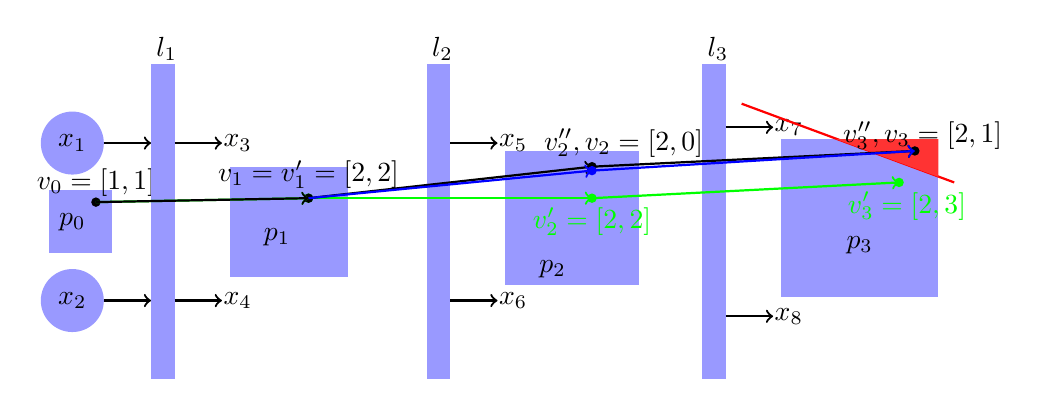
\begin{tikzpicture}
    \fill[blue!40!white] (3,3) circle (4mm);
    \fill[blue!40!white] (3,3) circle (0mm) node[color=black] {$x_1$};
    \fill[blue!40!white] (3,1) circle (4mm);
    \fill[blue!40!white] (3,1) circle (0mm) node[color=black] {$x_2$};
    \fill[blue!40!white] (2.7,1.6) rectangle (3.5,2.4);
    \fill[blue!40!white] (3,2) circle (0mm) node[color=black] {$p_0$};
    \fill[black] (3.3,2.25) circle (.6mm);
    \fill[blue!40!white] (3.3,2.5) circle (0mm) node[color=black] {$v_0 = [1,1]$};
    
    \draw[thick,->] (3.4,3) -- (4,3);
    \draw[thick,->] (3.4,1) -- (4,1);
    \fill[blue!40!white] (4,0) rectangle (4.3,4);
    \fill[blue!40!white] (5,1.3) rectangle (6.5,2.7);
    \fill[blue!40!white] (5.6,1.8) circle (0mm) node[color=black] {$p_1$};
    \draw[thick,->] (4.3,3) -- (4.9,3);
    \draw[thick,->] (4.3,1) -- (4.9,1);
    \fill[blue!40!white] (5.1,3) circle (0mm) node[color=black] {$x_3$};
    \fill[blue!40!white] (5.1,1) circle (0mm) node[color=black] {$x_4$};
    \fill[green] (6,2.3) circle (.6mm);
    \fill[black] (6,2.3) circle (.6mm);
    \fill[blue!40!white] (6,2.6) circle (0mm) node[color=black] {$v_1=v'_1=[2,2]$};
    % \fill[blue!40!white] (6,2) circle (0mm) node[color=green] {$v'_1$};
    \fill[blue!40!white] (4.2,4.2) circle (0mm) node[color=black] {$l_1$};

    \fill[blue!40!white] (7.5,0) rectangle (7.8,4);
    \fill[blue!40!white] (8.5,1.2) rectangle (10.2,2.9);
    \fill[blue!40!white] (9.1,1.4) circle (0mm) node[color=black] {$p_2$};
    \draw[thick,->] (7.8,3) -- (8.4,3);
    \draw[thick,->] (7.8,1) -- (8.4,1);
    \fill[blue!40!white] (8.6,3) circle (0mm) node[color=black] {$x_5$};
    \fill[blue!40!white] (8.6,1) circle (0mm) node[color=black] {$x_6$};
    \fill[green] (9.6,2.3) circle (.6mm);
    \fill[black] (9.6,2.7) circle (.6mm);
    \fill[blue!40!white] (10,3) circle (0mm) node[color=black] {$v''_2,v_2=[2,0]$};
    \fill[blue!40!white] (9.6,2) circle (0mm) node[color=green] {$v'_2 = [2,2]$};
    \fill[blue!40!white] (7.7,4.2) circle (0mm) node[color=black] {$l_2$};


    \fill[blue!40!white] (11,0) rectangle (11.3,4);
    \fill[blue!40!white] (12,1.05) rectangle (14,3.05);
    \fill[blue!40!white] (13,1.7) circle (0mm) node[color=black] {$p_3$};
    \draw[thick,->] (11.3,3.2) -- (11.9,3.2);
    \draw[thick,->] (11.3,.8) -- (11.9,.8);
    \fill[blue!40!white] (12.1,3.2) circle (0mm) node[color=black] {$x_7$};
    \fill[blue!40!white] (12.1,.8) circle (0mm) node[color=black] {$x_8$};
    \draw[red, thick] (14.2,2.5) -- (11.5,3.5);
    \fill[red!80!white] (12.7,3.05) -- (14,2.57) -- (14,3.05) -- cycle;
    \fill[black] (13.7,2.9) circle (.6mm);
    \fill[green] (13.5,2.5) circle (.6mm);
    \fill[blue!40!white] (13.8,3.1) circle (0mm) node[color=black] {$v''_3,v_3=[2,1]$};
    \fill[blue!40!white] (13.6,2.2) circle (0mm) node[color=green] {$v'_3 = [2,3]$};
    \fill[blue!40!white] (11.2,4.2) circle (0mm) node[color=black] {$l_3$};

    \draw[thick,->,green] (3.3,2.25)  -- (6, 2.3);
    \draw[thick,->,green] (6,2.3)  -- (9.6, 2.3);
    \draw[thick,->,green] (9.6, 2.3) -- (13.5, 2.5);

    \draw[thick,->,black] (3.3,2.25)  -- (6, 2.3);
    \draw[thick,->,black] (6,2.3)  -- (9.6, 2.7);
    \draw[thick,->,black] (9.6, 2.7) -- (13.7, 2.9);



    %Following lines are for blue line
    % \draw[thick,->,blue] (3.3,2.25)  -- (6, 2.3);
    \fill[blue] (9.6,2.65) circle (.6mm);
    \draw[thick,->,blue] (6,2.3)  -- (9.6, 2.65);
    \draw[thick,->,blue] (9.6, 2.65) -- (13.7, 2.9);
    % \fill[blue!40!white] (9.9,2.6) circle (0mm) node[color=blue] {$v''_2 = [2,0]$};

\end{tikzpicture}

\end{document}
